\section{Entropy: Is It Possible?}

\begin{comment}
This lab is more of a worksheet than it is a lab.  But I've used versions of if in my 132 classes for a while, so I thought it was time to include it here in the lab manual for others as well.  --Matt Trawick, 1/2016

\end{comment}

\makelabheader %(Space for student name, etc., defined in master.tex)

\vspace{0.2in}
\textbf{Introduction} 

We are all familiar with the idea that a closed system tends to evolve from an ordered state to a disordered state.  For example, when you put cream into a mug of coffee, the cream tends to disperse: the mug evolves from an ``ordered'' state, with seperate regions of pure cream and black coffee, to a ``disordered'' state with the two mixed together.  The reverse process, spontaneous separation back into pure cream and black coffee, will never happen.

We also know intuitively that heat will always flow from a hot object to a cold object: when you put a hot brick in contact with a cold brick, you end up with two luke-warm bricks.  The reverse process, two luke-warm bricks spontaneously evolving to one hot brick and one cold brick, won't happen.  

In both of the examples above, the ``disorder'' (or ``dispersal'') of the system increases.  We quantify that disorder using entropy, $S$, and for any real process, $\Delta S \geq 0$.  In the context of heat transfer, the change in entropy $\Delta S$ of an object is given by 
\begin{displaymath}
\Delta S = \frac{\Delta Q}{T},
\end{displaymath}
where $\Delta Q$ is the heat energy into the object.  

\vspace{0.3 in}
\textbf{Activity 1: Just Heat Transfer}

Consider the previous example of the hot and cold bricks, illustrated below.

\begin{center}
\vspace{-0.2 in}
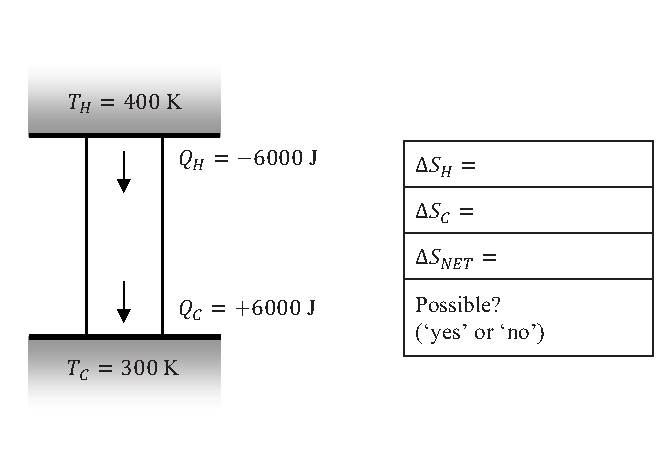
\includegraphics[width=0.5\textwidth]{entropy_is_it_possible/fig1.eps}
\vspace{-0.2 in}
\end{center}

(a) Use the expression for $\Delta S$ to fill in the table to the right of the figure with $\Delta S_H$ and $\Delta S_C$ for the hot and cold bricks.  Be careful with the signs for $Q_H$ and $Q_C$!  (We've dropped the ``$\Delta$'' from our notation for simplicity.)  Note that we're assuming here that both bricks are large enough that their temperatures remain roughly constant throughout the process; transferring 6000 Joules doesn't make a lot of difference to them.  Our lingo here is that those bodies are hot and cold ``reservoirs.''   
\answerspace{0.2 in}

(b) The net change in entropy $\Delta S_{NET}$ is the sum of $\Delta S_H$ and $\Delta S_C$.  Based on the sign of $\Delta S_{NET}$, is the process pictured above one that is actually possible in nature?
\answerspace{0.6 in}

\pagebreak[2]
Now consider the reverse process:

\begin{center}
\vspace{-0.2 in}
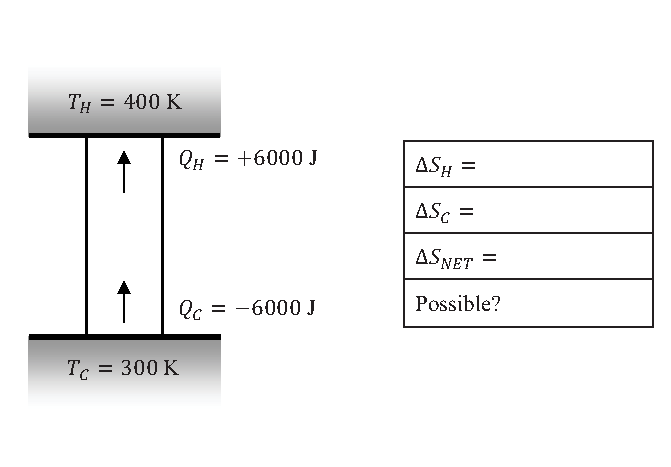
\includegraphics[width=0.5\textwidth]{entropy_is_it_possible/fig2.eps}
\vspace{-0.2 in}
\end{center}

(c) Fill in the table to the right of the figure above.   Could this process actually occur?  How do you know?
\answerspace{0.6 in}

\textbf{Activity 2: Extracting Work: Heat Engines}

There are many ways you can convert mechanical work $W$ into heat energy $Q$.  You can rub your hands together quickly to heat them with friction, or you can mechanically turn a generator to produce electricity and use it to power an electric heater.  Your experience tells you that using either of these methods to heat up a single brick doesn't break any physical laws.  In fact, the work $W$ you do has no direct bearing on $S_{NET}$, though the amount of heat $Q$ transferred does.

\begin{center}
\vspace{-0.2 in}
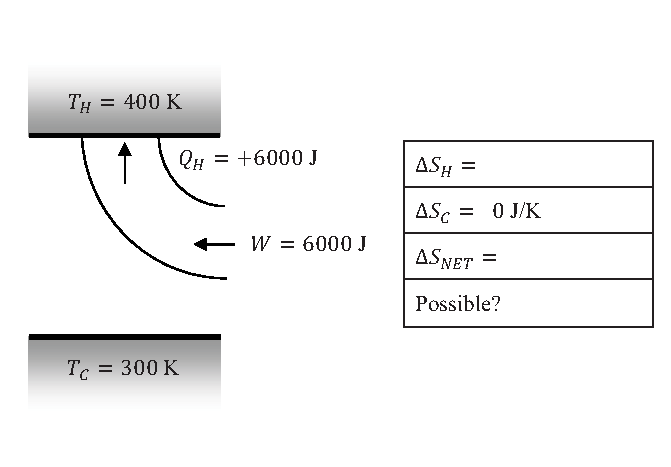
\includegraphics[width=0.5\textwidth]{entropy_is_it_possible/fig3.eps}
\vspace{-0.2 in}
\end{center}

(a) Fill in the table to the right of the figure.  Is the sign for $\Delta S$ consistent with whether this process can actually occur?
\answerspace{0.6 in}

\pagebreak[3]
Now consider the reverse process, in which heat energy is extracted from an object, and all of it is somehow transformed into useful mechanical work, like lifting some weights or generating electricity to do something else.

\begin{center}
\vspace{-0.2 in}
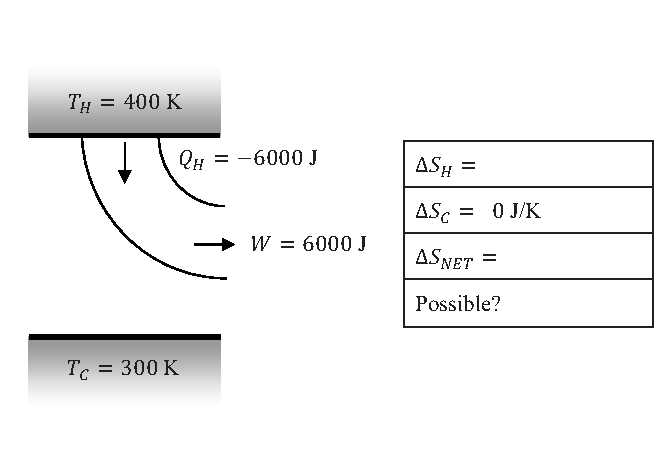
\includegraphics[width=0.5\textwidth]{entropy_is_it_possible/fig4.eps}
\vspace{-0.2 in}
\end{center}

(b) Fill in the table to the right of the figure.  Could this process actually occur? 
\answerspace{0.2 in}

But wait a second!  We \textit{know} that you can use heat from burning coal or from a nuclear reaction to turn water into steam, and that the steam can be used to turn a turbine on a generator.  This is where most of our electricity comes from!  \textit{Surely this is possible, right?}  The catch is that not all of the heat energy can be converted to work.  Some the heat from the steam must be transferred to a cold body, typically either to the atmosphere or to a large body of water.  

In the figure below, enough coal is burned to generate 6000 J of heat in a reservoir of steam.  Of the 6000 J transferred from the hot steam, 4800 J is dumped into the colder atmosphere, in the form of heat pouring from a smokestack, say.   

\begin{center}
\vspace{-0.3 in}
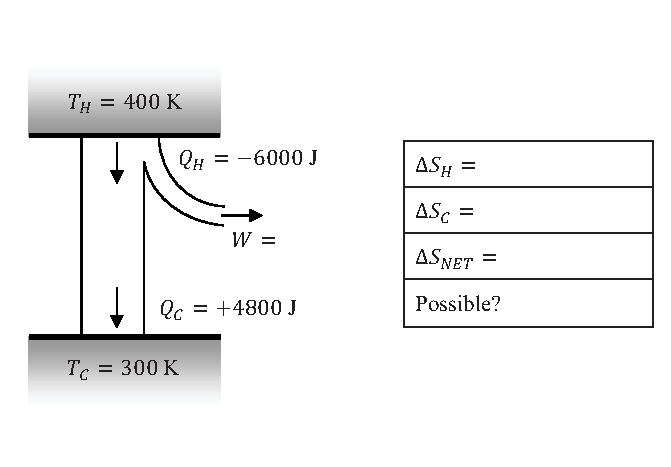
\includegraphics[width=0.5\textwidth]{entropy_is_it_possible/fig5.eps}
\vspace{-0.3 in}
\end{center}

(c) Fill in the table to the right of the figure, including the amount of work $W$ that is extracted.  Could the process actually occur, as shown?
\answerspace{0.2 in}

(d) The limiting case of a process that's theoretically \textit{just barely} possible is $\Delta S_{NET} = 0$.  Suppose that 6000 J is transferred from the hot reservoir.  What's the limit for the minimum $Q_C$ that must be transferred to the cold reservoir?
\answerspace{0.2 in}

(e) If  6000 J is transferred from the hot reservoir, what is the maximum work $W$ that can be extracted from the process?
\answerspace{0.2 in}

\pagebreak[2]
(f) Write a general expression for the maximum ratio of $W/Q_H$, in terms of only $T_H$ and $T_C$.  (Hint: start by writing $\Delta S = 0$ in terms of $Q_H$, $Q_C$, and the temperatures of the reservoirs.  Then use the idea of conservation of energy to write $Q_C$ in terms of $Q_H$ and $W$.)
\answerspace{1.5 in}

\textbf{Activity 3: Heating and Cooling Your House: Refrigerators and Heat Pumps}

Think of a hot summer day, when it's $100^\circ$F outside and your house is a stuffy $85^\circ$F inside.  

(a) If you open a window, is it possible that heat will spontaneously be transferred from inside your house to outside your house?  Why or why not?  (A diagram might help.  See Activity 1 if you're not sure.)
\answerspace{1.2 in}

(b) Is it possible to simply transform some thermal energy $Q$ from inside your house into mechanical work $W$?  Why or why not?  (Again, a diagram might help.  See Activity 2 if you're not sure.)
\answerspace{1.2 in}

The way to actually cool your house is to transfer some heat energy to the outside with the help of additional mechanical work, as shown below.  This is how an air conditioner works (more generally called a ``refrigerator'').

\begin{center}
\vspace{-0.3 in}
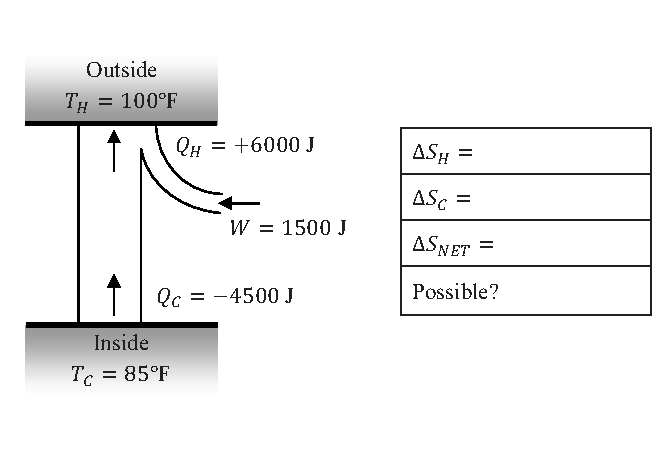
\includegraphics[width=0.5\textwidth]{entropy_is_it_possible/fig6.eps}
\vspace{-0.4 in}
\end{center}

(c) Fill in the table to the right of the figure, including the heat energy $Q_H$, to show that the situation above is possible for the quantities given.  (Yes, you have to convert from Fahrenheit to Kelven.)
\answerspace{0.2 in}

\pagebreak[2]
Finally, suppose you want to heat your house in the winter when it's $65^\circ$F inside and $50^\circ$F outside.  The diagrams below show two possible ways to do it.  On the left is a simple space heater, in which work is converted to heat energy.  On the right is a ``heat pump,'' which is basically the same as the air conditioner, but with the inside and outside flipped.  In each case, you are putting 6000 J of heat energy into the house.

\begin{center}
\vspace{-0.2 in}
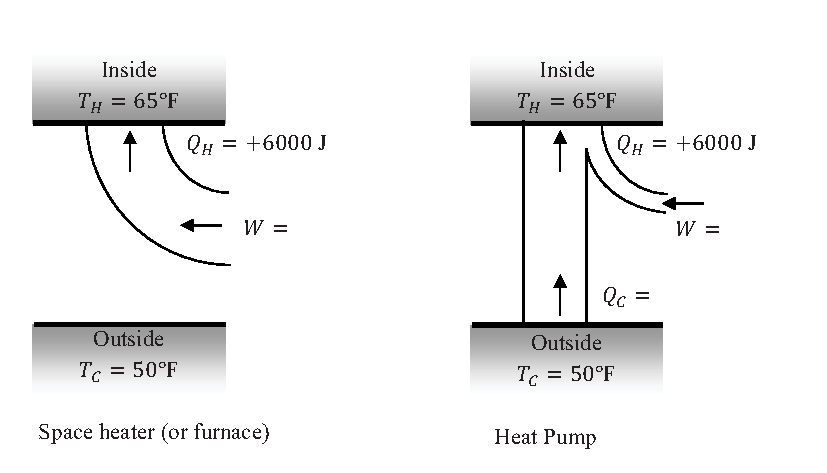
\includegraphics[width=0.5\textwidth]{entropy_is_it_possible/fig7.eps}
\vspace{-0.1 in}
\end{center}

(d) The theoretical maximum efficiency of the heat pump would be when $\Delta S_{NET}=0$.  What would $Q_C$ need to be then?
\answerspace{1.2 in}

(e) If the heat pump is at that maximum theoretical efficiency, how much work $W$ is required for $Q_H = 6000$ J?
 \answerspace{0.6 in}

(f) By contrast, how much work $W$ does the simple space heater need to do the same job? 
\answerspace{0.4 in}

(g) How cool is that?
\answerspace{0.4 in}

(h) If the outside temperature were colder, would the advantage of the heat pump over the simple space heater increase or decrease? 
\answerspace{0.4 in}

In real life, heat pumps aren't quite as efficient as the maximum theoretical efficiency you assumed here.  And as you noted above, they get worse when the outside temperature gets colder.  (They also usually run on electricity, and the cost per Joule for electrical power is generally higher than for natural gas.)  Nevertheless, houses in moderate climates like Virginia and further south often have heat pumps, sometimes in addition to traditional gas furnaces.  The heat pump warms the house economically in the fall and spring, and a thermostat trips the gas furnace to kick on when the outside temperature falls below about $40^\circ$F.

